\documentclass[12pt,letterpaper]{article}
\usepackage[utf8]{inputenc}
\usepackage[spanish]{babel}
\usepackage{graphicx}
\usepackage[left=2cm,right=2cm,top=2cm,bottom=2cm]{geometry}
\usepackage{graphicx} % figuras
\usepackage{hyperref}
% \usepackage{subfigure} % subfiguras
\usepackage{float} % para usar [H]
\usepackage{amsmath}
%\usepackage{txfonts}
\usepackage{stackrel} 
\usepackage{multirow}
\usepackage{enumerate} % enumerados
\renewcommand{\labelitemi}{$-$}
\renewcommand{\labelitemii}{$\cdot$}
% \author{}
% \title{Caratula}
\begin{document}

% Fancy Header and Footer
% \usepackage{fancyhdr}
% \pagestyle{fancy}
% \cfoot{}
% \rfoot{\thepage}
%

% \usepackage[hidelinks]{hyperref} % CREA HYPERVINCULOS EN INDICE

% \author{}
\title{Caratula}

\begin{titlepage}
\begin{center}
\large{UNIVERSIDAD PRIVADA-DE-TACNA}\\
\vspace*{-0.025in}
\begin{figure}[htb]
\begin{center}

\includegraphics[width=8cm]{./Imagenes/logo}
\end{center}
\end{figure}
\vspace*{0.15in}
INGENIERIA DE SISTEMAS  \\

\vspace*{0.5in}
\begin{large}
TITULO:\\
\end{large}

\vspace*{0.1in}
\begin{Large}
\textbf{TRABAJO FINAL DE UNIDAD} \\
\end{Large}

\vspace*{0.3in}
\begin{Large}
\textbf{CURSO:} \\
\end{Large}

\vspace*{0.1in}
\begin{large}
BASE DE DATOS II\\
\end{large}

\vspace*{0.3in}
\begin{Large}
\textbf{DOCENTE(ING):} \\
\end{Large}

\vspace*{0.1in}
\begin{large}
 Patrick Cuadros Quiroga\\
\end{large}

\vspace*{0.2in}
\vspace*{0.1in}
\begin{large}
Integrantes: \\
\begin{flushleft}
Arlyn Cotrado Coaquira		\hfill	(2016054466) \\
Yaneth Virginia Aquino Huallpa		\hfill	(2017059286) \\
Sharon Sosa Bedoya            	\hfill	(2016054460) \\
Marlon Villegas Arando	\hfill	(2015053890) \\
\end{flushleft}
\end{large}
\end{center}

\end{titlepage}


\tableofcontents % INDICE
\thispagestyle{empty} % INDICE SIN NUMERO
\newpage
\setcounter{page}{1} % REINICIAR CONTADOR DE PAGINAS DESPUES DEL INDICE

\section{PROBLEMA} 

\par El siguiente trabajo se desarrolla con el Sistema de Gestion de Gimnasio, el cual  busca que el gimnasio adquiera una mejor organización ahorrando tiempo y trabajo para recolección de información, permitiendo: \\
•	La gestión de los entrenadores, miembros, planes, usuarios.\\
•	Gestión de las clases que se brinden asignando un entrenador a una clase, evitando el cruce de horarios en diferentes sucursales.\\
•	La venta de distintos tipos de planes.\\
•	La realización de reportes sobre las ventas realizadas del día, del mes, y sobre los clientes correspondientes a cada local.\\
•	El sistema permitirá realizar la autentificación de los usuarios.\\

\par La motivación principal de este proyecto es que el gimnasio adquiera una mejor organización, lo que le permitirá realizar sus tareas sin inconvenientes.

\section{MARCO TEORICO} 

\par 

\subsection{API REST}
	\par Ha pasado más de una década desde que Roy Fielding, un científico informático estadounidense y uno de los autores principales de la especificación HTTP, introdujo Representational State Transfer (REST) como un estilo de arquitectura. A lo largo de los años, REST ha ganado impulso gracias a su popularidad para la creación de servicios web.\\
Al no tener estado, y al crear identificadores únicos para permitir el almacenamiento en caché, la creación de capas y la capacidad de lectura, las API REST hacen uso de los verbos HTTP existentes (GET, POST, PUT y DELETE) para crear, actualizar y eliminar nuevos recursos. El término REST se usa con frecuencia para describir cualquier URL que devuelva JSON en lugar de HTML.[3]
\subsection{Entity Framework}
	\par Entity Framework es un marco de ORM de código abierto para aplicaciones .NET admitidas por Microsoft. Permite a los desarrolladores trabajar con datos utilizando objetos de clases específicas del dominio sin centrarse en las tablas y columnas de la base de datos subyacente donde se almacenan estos datos. Con el Entity Framework, los desarrolladores pueden trabajar en un nivel más alto de abstracción cuando tratan con datos, y pueden crear y mantener aplicaciones orientadas a datos con menos código en comparación con las aplicaciones tradicionales.[2]\\
\\Su arquitectura:
\begin{figure}[H]
\begin{center}
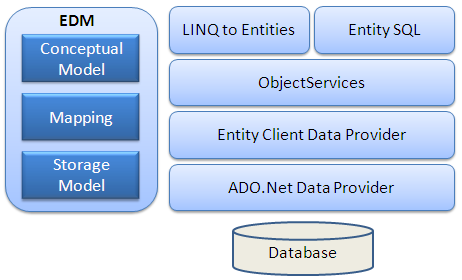
\includegraphics[width=9cm]{./Imagenes/ef-architecture}
\end{center}
\end{figure}

\subsection{ Consultas LINQ}
	\par Permite consultar cualquier objeto  enumerable en ADO.NET mediante el uso del modelo de programación de Language-Integrated Query (LINQ) [1] para recuperar datos de la base de datos subyacente. El proveedor de la base de datos traducirá estas consultas LINQ al lenguaje de consulta específico de la base de datos (por ejemplo, SQL para una base de datos relacional).\\
Hay 3 tecnologias ADO.NET LINQ distintas:
\begin{itemize}
	\item LINQ to DataSet: proporciona una capacidad de consulta mas rica y optimizada sobre DataSet.
	\item LINQ to SQL: permite consultar directamente los esquemas de las base de datos de SQL Server.
	\item LINQ to Entities: permite consultar Entity Data Model.
\end{itemize}

\subsection{Pruebas Unitarias}
	\par Las pruebas unitarias son la mejor forma de probaar el codigo de una aplicación a lo largo de su desarrollo. Estas pruebas permiten asegurar que losmétodos devuelven resultados correctos, teniendo en cuenta los argumentos que se le pasan y, además, se pueden utilizar para hacer Test Driven Development. Se trata de una técnica en la que se escriben antes que las clases y los métodos.[4]\\
 No obstante, tras realizar la integración con otros módulos deberá revisarse de nuevo la interfaz.
\section{DESARROLLO} 

\subsection{Analisis}
\begin{itemize}
	\item Casos de Uso
	\begin{figure}[H]
		\begin{center}
			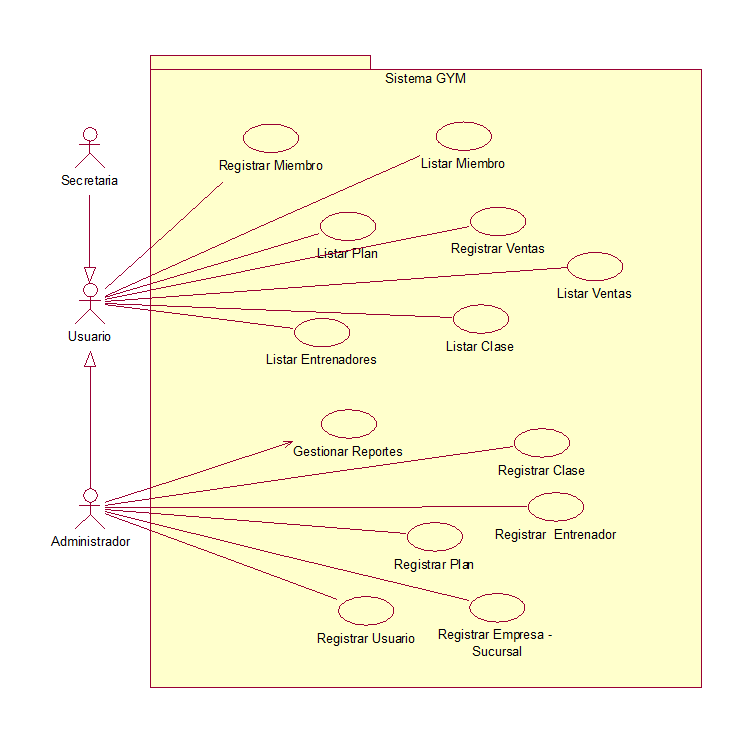
\includegraphics[width=15cm]{./Imagenes/CasosDeUso}
		\end{center}
	\end{figure}
\end{itemize}


\subsection{Diseño}
\begin{itemize}
	\item Diagrama de Clases
\begin{center}
	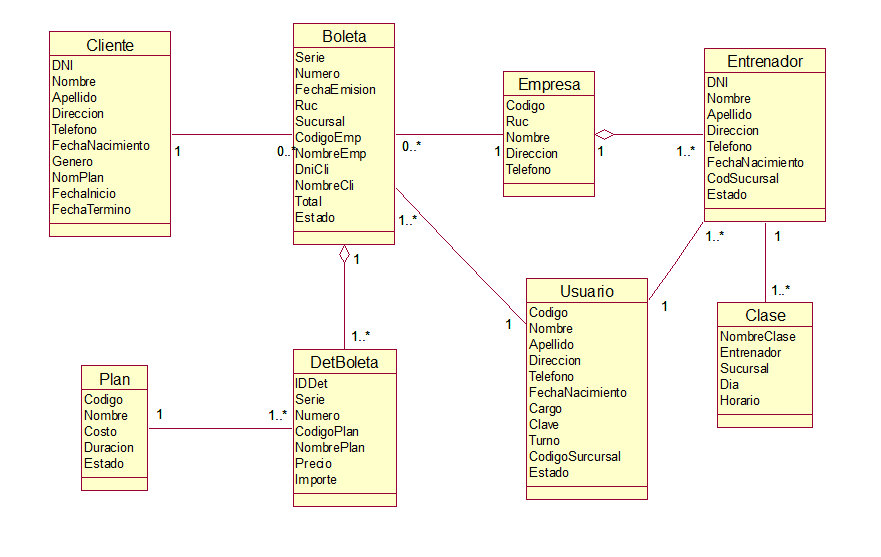
\includegraphics[width=15cm]{./Imagenes/DiagramaClases}
\end{center}
	\item Modelo Entidad Relación
\begin{figure}[H]
		\begin{center}
			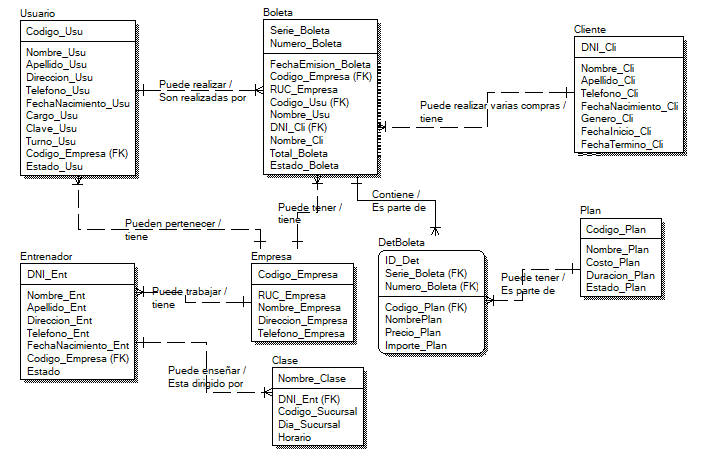
\includegraphics[width=17cm]{./Imagenes/EntidadRelacion}
		\end{center}
	\end{figure}
\end{itemize}



\subsection{Pruebas}
Las pruebas realizadas fueron las siguientes:
\begin{itemize}
	\item ObtenerAlEntrenadorPorCodigo 
\begin{center}
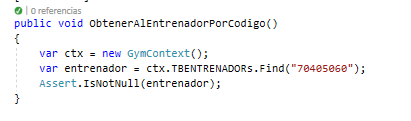
\includegraphics[width=15cm]{./Imagenes/prueba1.png}
\end{center}
Sentencia SQL generada:
\begin{center}
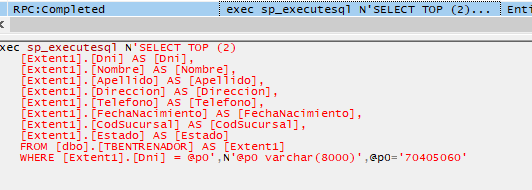
\includegraphics[width=15cm]{./Imagenes/profile1.png}
\end{center}
	\item AgregarDosPlanesdeGimnasio
\begin{center}
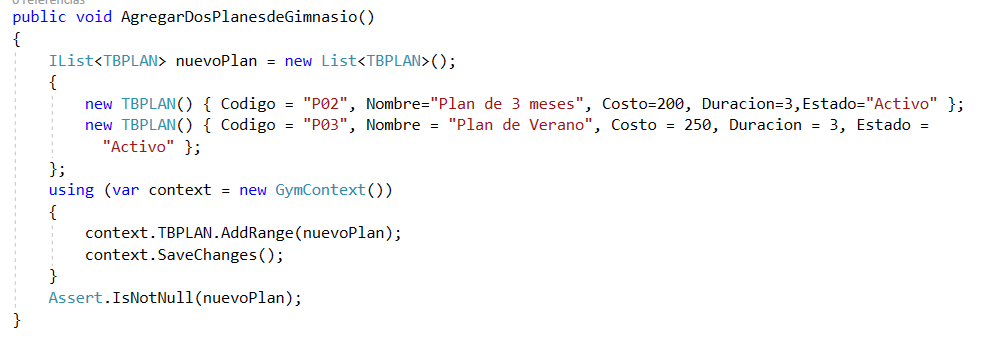
\includegraphics[width=17cm]{./Imagenes/prueba2.png}
\end{center}
Sentencia SQL generada:
\begin{center}
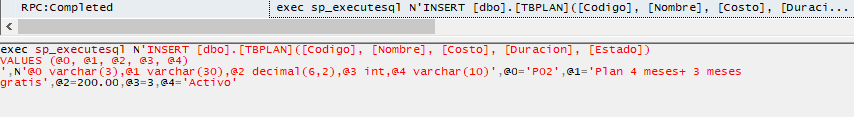
\includegraphics[width=17cm, height=3cm]{./Imagenes/profile2-1.png}
\end{center}
\begin{center}
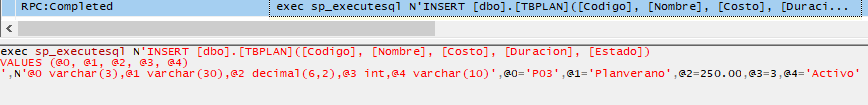
\includegraphics[width=17cm, height=3cm]{./Imagenes/profile2-2.png}
\end{center}
	\item ObtenerListaDeClasesPorNombreAscendiente
\begin{center}
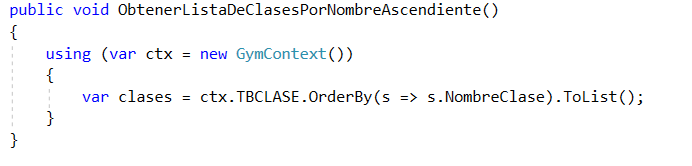
\includegraphics[width=15cm]{./Imagenes/prueba3.png}
\end{center}
Sentencia SQL generada:
\begin{center}
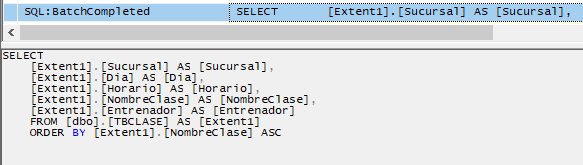
\includegraphics[width=15cm]{./Imagenes/profile3.png}
\end{center}
	\item BuscarTodaslasBoletasPorEmpleado
\begin{center}
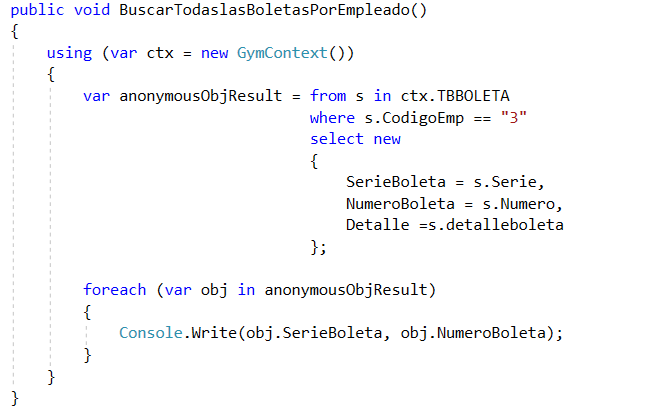
\includegraphics[width=15cm]{./Imagenes/prueba4.png}
\end{center}
Sentencia SQL generada:
\begin{center}
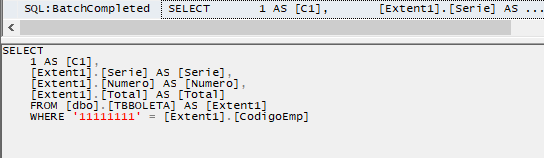
\includegraphics[width=15cm]{./Imagenes/profile4.png}
\end{center}
	\item EliminarUnPlanDeGimnasioPorCodigo
\begin{center}
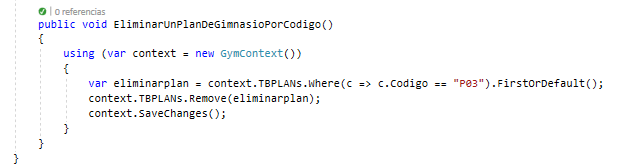
\includegraphics[width=15cm]{./Imagenes/prueba5.png}
\end{center}
Sentencia SQL generada:
\begin{center}
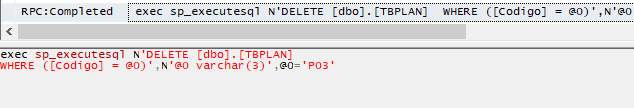
\includegraphics[width=15cm]{./Imagenes/profile5.png}
\end{center}
\end{itemize}
\subsection{API/Postman}

             \begin{center}
			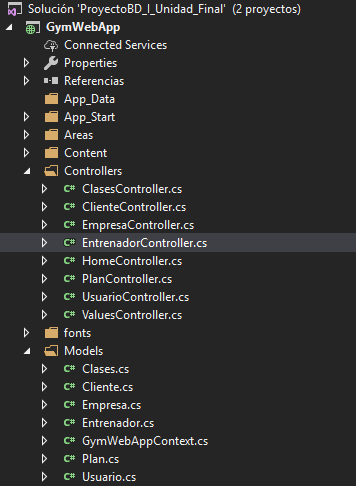
\includegraphics[width=10cm]{./Imagenes/1}
             \end{center}
\begin{itemize}
\item Del controlador Cliente, hacemos clic en POST Cliente para agregar un registro.
    \begin{center}
			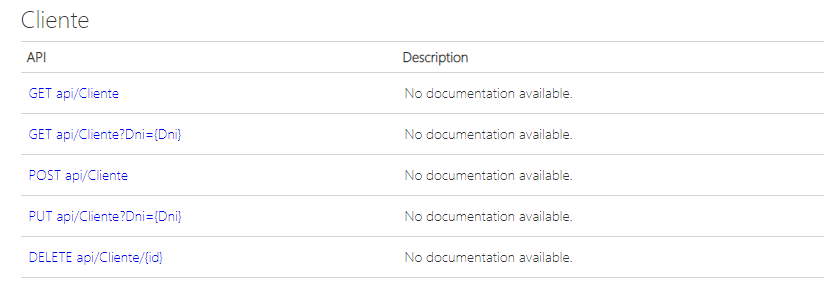
\includegraphics[width=16cm]{./Imagenes/cl}
             \end{center}
Copiamos el formato de la cadena, y luego la pegamos en Postman, donde agregaremos un nuevo cliente.
    \begin{center}
			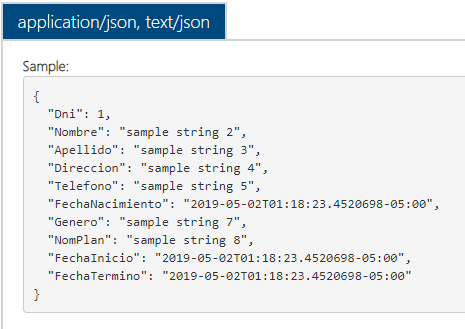
\includegraphics[width=10cm]{./Imagenes/clp}
             \end{center}
 \begin{center}
			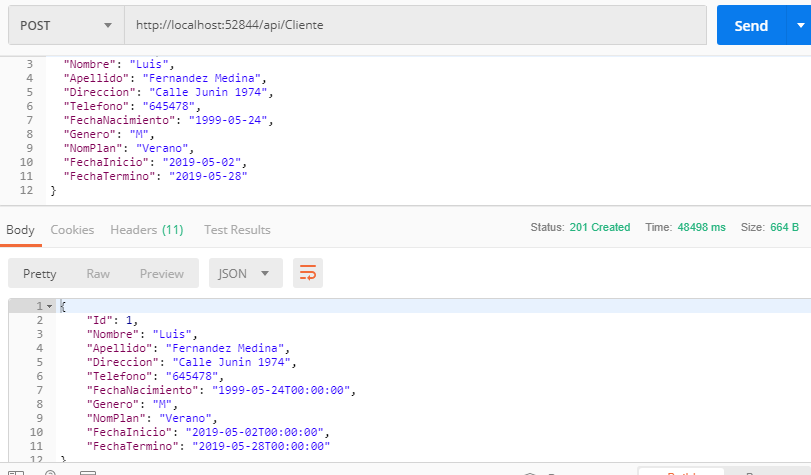
\includegraphics[width=15cm]{./Imagenes/pcl}
             \end{center}
\item Comprobamos que ha sido agregado el nuevo registro en la tabla con GET.
 \begin{center}
			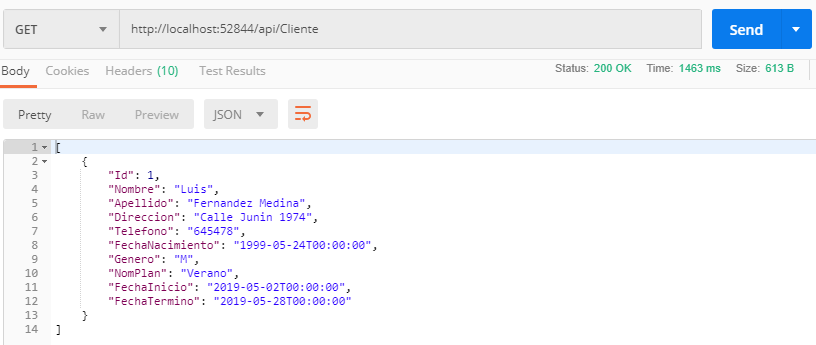
\includegraphics[width=15cm]{./Imagenes/gcl}
             \end{center}
\item Del controlador Usuario, hacemos clic en POST Usuario para agregar un registro.
 \begin{center}
			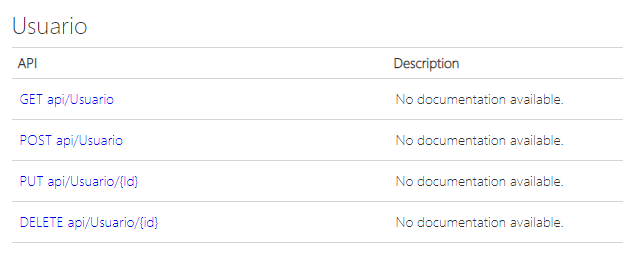
\includegraphics[width=14cm]{./Imagenes/us}
             \end{center}
Copiamos el formato de la cadena, y luego la pegamos en Postman, donde agregaremos un nuevo usuario.
 \begin{center}
			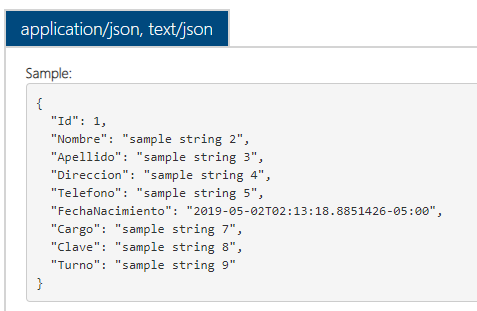
\includegraphics[width=10cm]{./Imagenes/pusu}
             \end{center}
 \begin{center}
			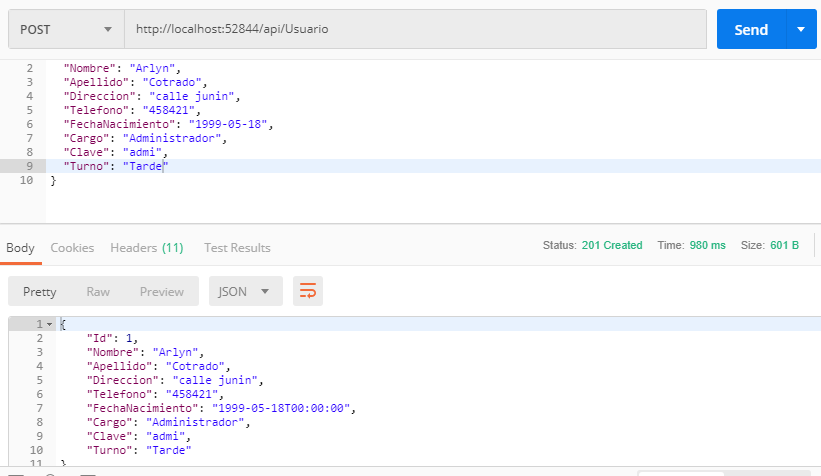
\includegraphics[width=15cm]{./Imagenes/usu}
             \end{center}
\item Del controlador Entrenador, hacemos clic en POST Entrenador para agregar un registro.
 \begin{center}
			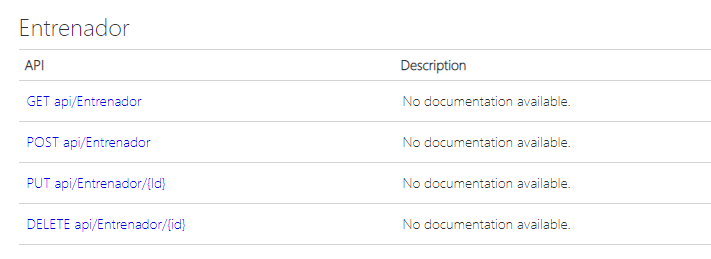
\includegraphics[width=15cm]{./Imagenes/ent}
             \end{center}
Copiamos el formato de la cadena, y luego la pegamos en Postman, donde agregaremos un nuevo entrenador.
 \begin{center}
			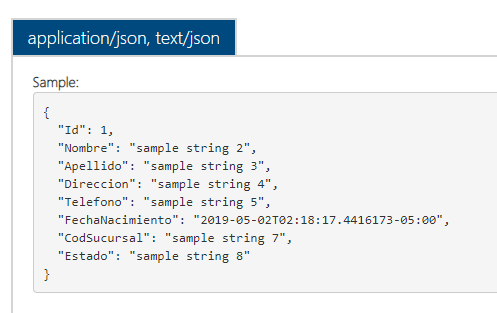
\includegraphics[width=10cm]{./Imagenes/e}
             \end{center}
 \begin{center}
			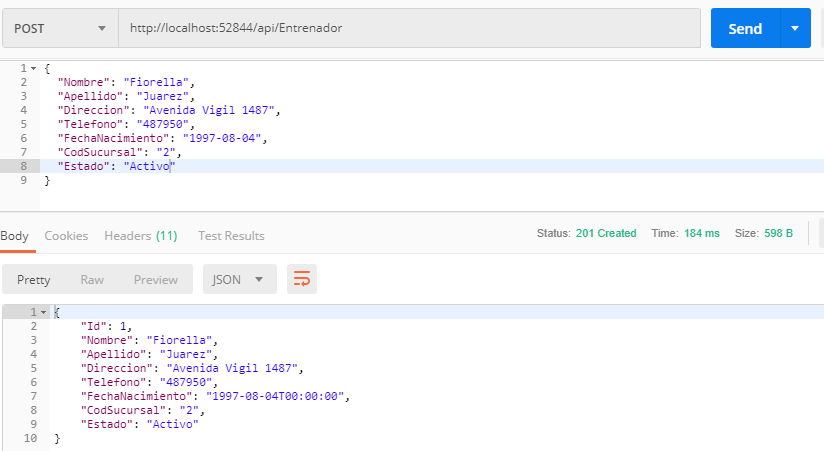
\includegraphics[width=15cm]{./Imagenes/pent}
             \end{center}
\item Del controlador Plan, hacemos clic en POST Plan para agregar un registro.
 \begin{center}
			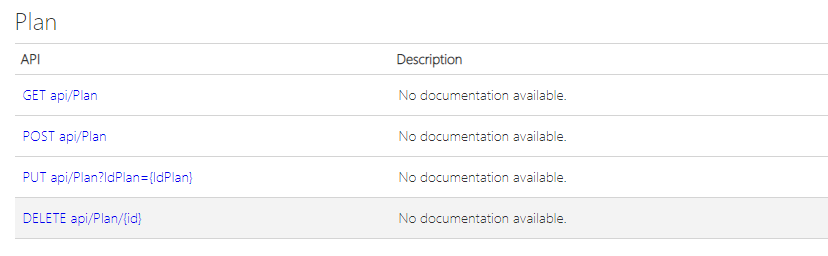
\includegraphics[width=15cm]{./Imagenes/plan}
             \end{center}
Copiamos el formato de la cadena, y luego la pegamos en Postman, donde agregaremos un nuevo plan.
 \begin{center}
			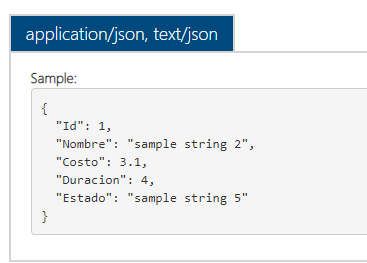
\includegraphics[width=8cm]{./Imagenes/p}
             \end{center}
 \begin{center}
			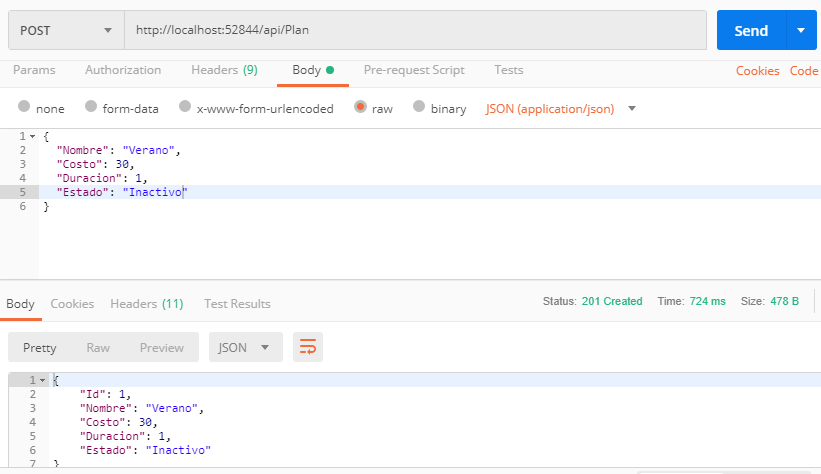
\includegraphics[width=15cm]{./Imagenes/pp}
             \end{center}
\item Del controlador Empresa, hacemos clic en POST Empresa para agregar un registro.
 \begin{center}
			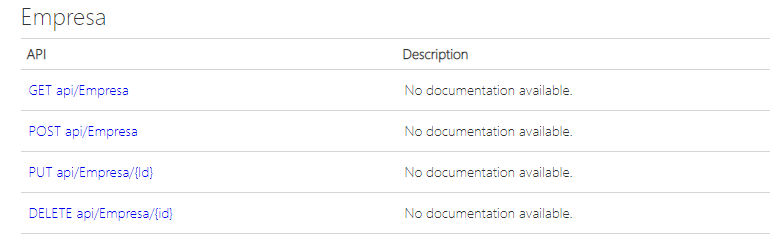
\includegraphics[width=15cm]{./Imagenes/emp}
             \end{center}
Copiamos el formato de la cadena, y luego la pegamos en Postman, donde agregaremos un nuevo empresa.
 \begin{center}
			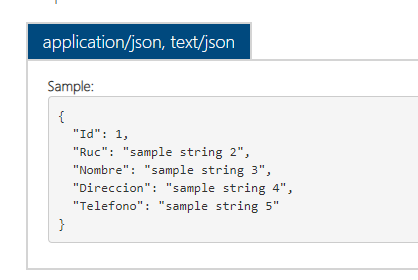
\includegraphics[width=10cm]{./Imagenes/em}
             \end{center}
 \begin{center}
			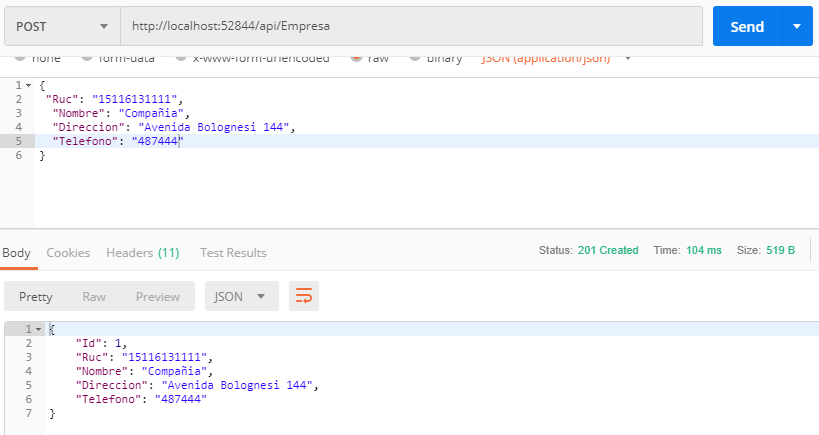
\includegraphics[width=15cm]{./Imagenes/pem}
             \end{center}

\end{itemize}



        
        
        


\section{REFERENCIAS} 


\end{document}
